\subsection{User Interface}
	\subsubsection{Overview}
	Our choose of Phonegap for cross compiling, gave us the possibility to use CSS and JavaScript to design our application. We were able to use existing libraries (CSS, html, etc.) in our code. The JavaScript library, jQuery mobile had touch-optimized layouts which were suitable for our application, both because of its good design and its simplicity. We therefore chose to use the jQuery mobile layout for our application.  

	\subsubsection{Choose of Template}
Artsdatabanken does have a webpage optimized for mobile phones, which also uses jQuery mobile. The customer wanted the application to have the same template as the webpage. To do that we used the CSS file from the webpage, in our application. By this way the application looked very similar to the mobile webpage. 
\begin{figure}[h]
 \begin{center}$
 \begin{array}{cc}
 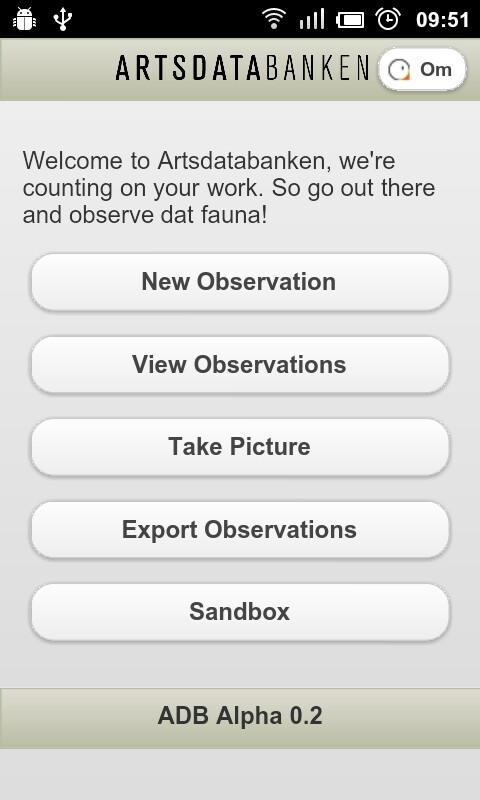
\includegraphics[width=0.5\textwidth]{sprints/ui/main.jpg} &
 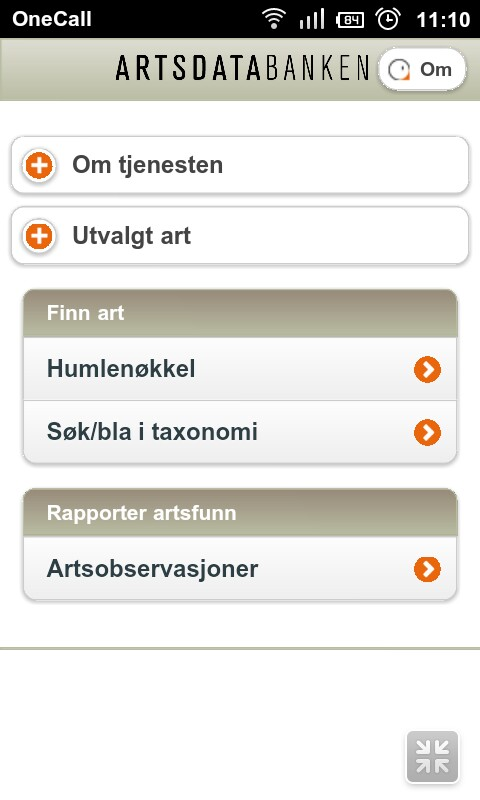
\includegraphics[width=0.5\textwidth]{sprints/ui/webpage.jpg}
 \end{array}$
 \end{center}
 \caption{Similarity of the application (left) and  the webpage (right). }
 \end{figure}



\newpage
\subsubsection{Preview of the UI with Screenshots}


\begin{figure}[h]
 \begin{center}$
 \begin{array}{cc}
 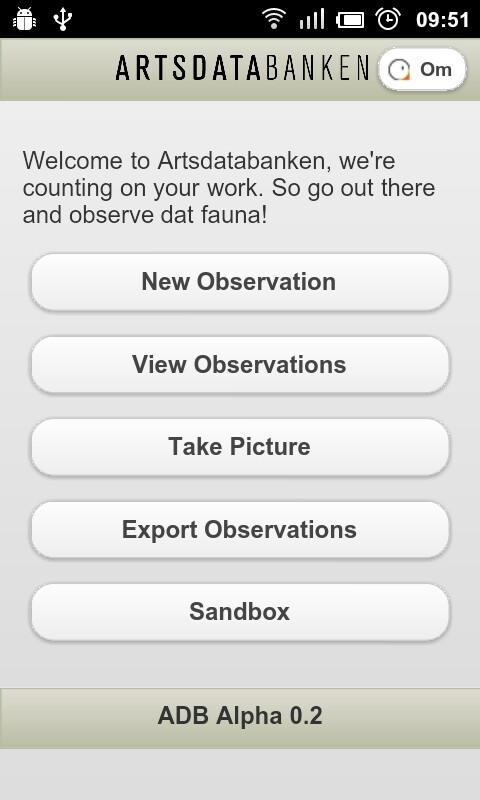
\includegraphics[width=0.5\textwidth]{sprints/ui/main.jpg} &
 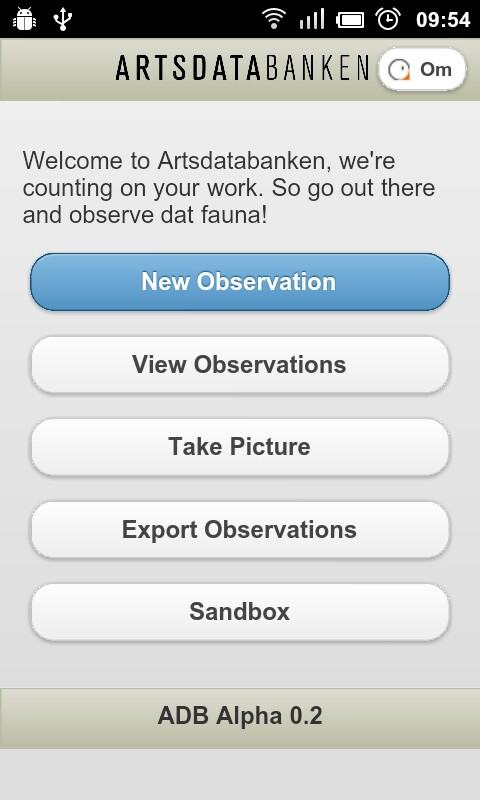
\includegraphics[width=0.5\textwidth]{sprints/ui/mainHover.jpg}
 \end{array}$
 \end{center}
 \caption{Main Screen, Right:Button Clicked }
 \end{figure}

\subparagraph{Main Screen}
Figure above shows the main screen of the application. The buttons are clear and the user can simply do a selection
When the user makes a selection, the selected button becomes blue and the user is gets sure he pressed the right button.  

\newpage
\begin{figure}[h]
 \begin{center}$
 \begin{array}{cc}
 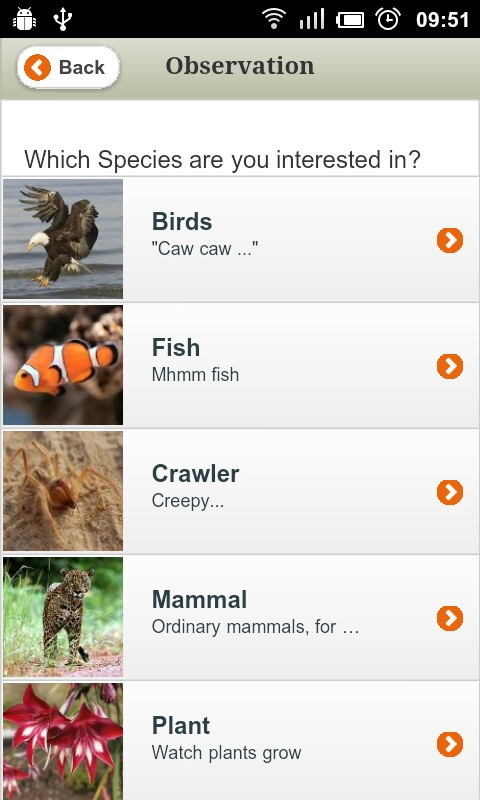
\includegraphics[width=0.5\textwidth]{sprints/ui/obs.jpg} &
 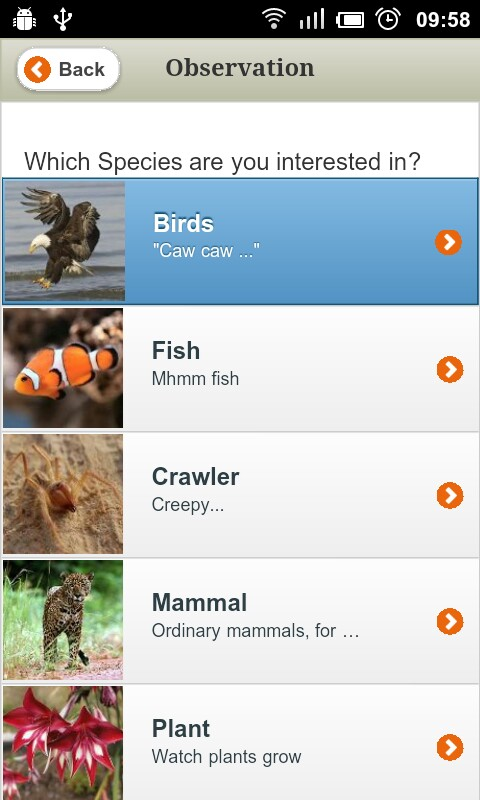
\includegraphics[width=0.5\textwidth]{sprints/ui/obsHover.jpg}
 \end{array}$
 \end{center}
 \caption{New Observation, Right:Button Clicked }
 \end{figure}

\subparagraph{New Observation}
After selecting New Observation, we get into the window displayed in figure 11. Here the user selects the Species.  Their names are displayed, with a picture on the side. More species are listed; the user needs to slide his finger to see those. 

The selection will give a feedback to the user, like in the main screen.

There is a back button on the top left. This button will lead the user to the previous window.


\newpage
\begin{figure}[h]
 \begin{center}$
 \begin{array}{cc}
 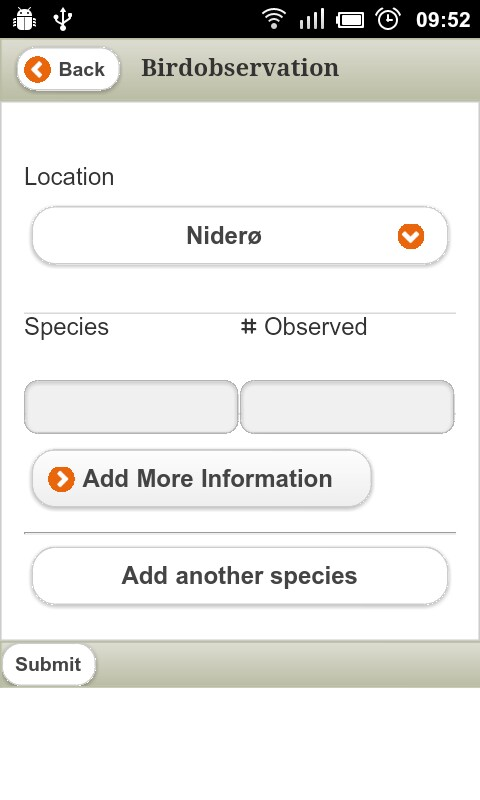
\includegraphics[width=0.5\textwidth]{sprints/ui/bird.jpg} &
 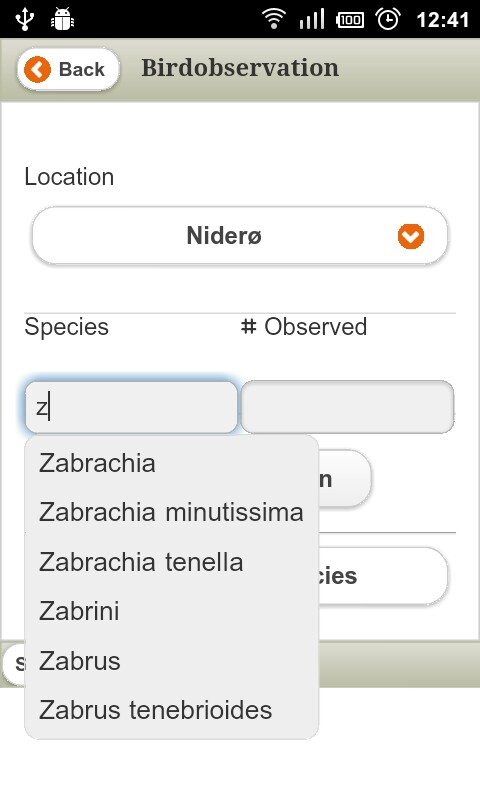
\includegraphics[width=0.5\textwidth]{sprints/ui/autocomp.jpg}
 \end{array}$
 \end{center}
 \caption{Bird Observation, Right:Auto-Complete field }
 \end{figure}

\subparagraph{Bird Observation}
After selecting the specie; bird, we get a new window (figure 12). This is the window where the user adds the information about the observation. 

The user can fill the fields easily by selecting the field he wants to fill. The selected field is marked with a blue shadow so the user knows which field is selected.  The specie field has an auto-complete function, which makes it simpler for the user to type the correct name. 

\newpage
\begin{figure}[h]
 \begin{center}$
 \begin{array}{cc}
 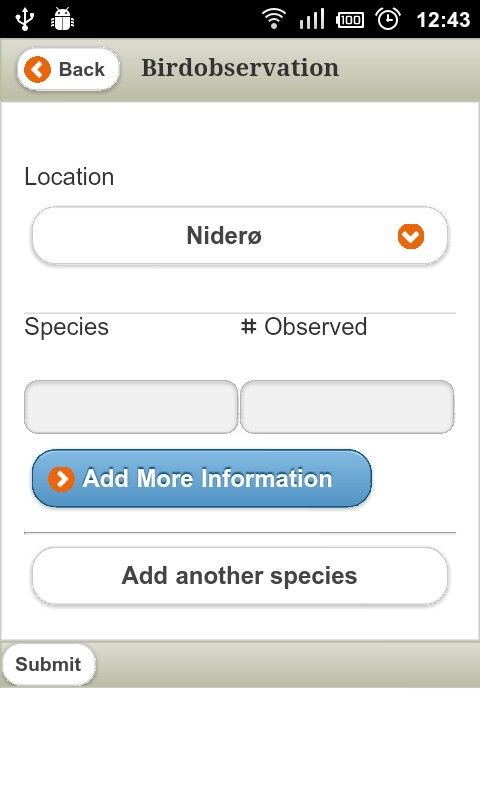
\includegraphics[width=0.5\textwidth]{sprints/ui/add_more.jpg} &
 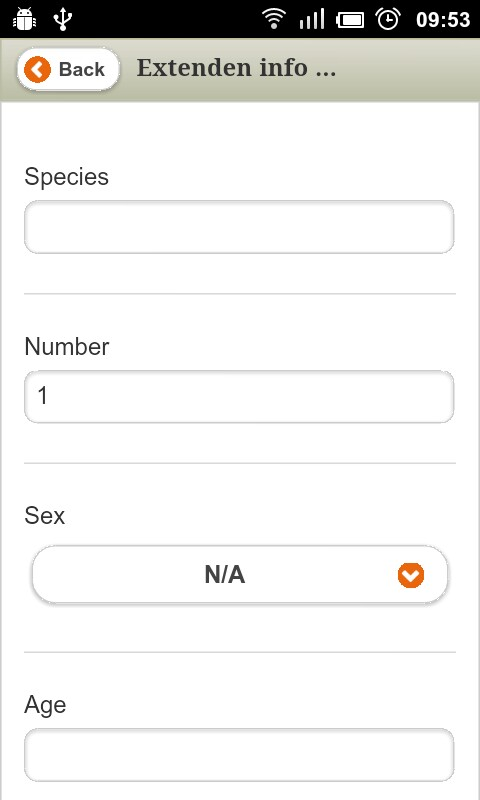
\includegraphics[width=0.5\textwidth]{sprints/ui/add_more2.jpg}
 \end{array}$
 \end{center}
 \caption{Add More Information, Right:New window after select }
 \end{figure}
\subparagraph{Add More information}
There are several buttons here for the user. If the user wants to add more information about the specie, the “Add More Information” button is selected. This leads to a new window (shown in figure 13).  To go back after entering new data, the user 
selects the back button.

\newpage
\begin{figure}[h]
 \begin{center}$
 \begin{array}{cc}
 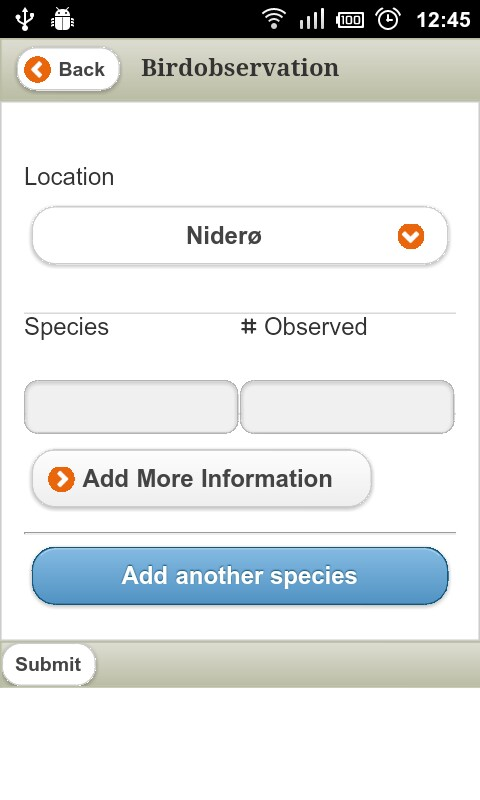
\includegraphics[width=0.5\textwidth]{sprints/ui/add_specie.jpg} &
 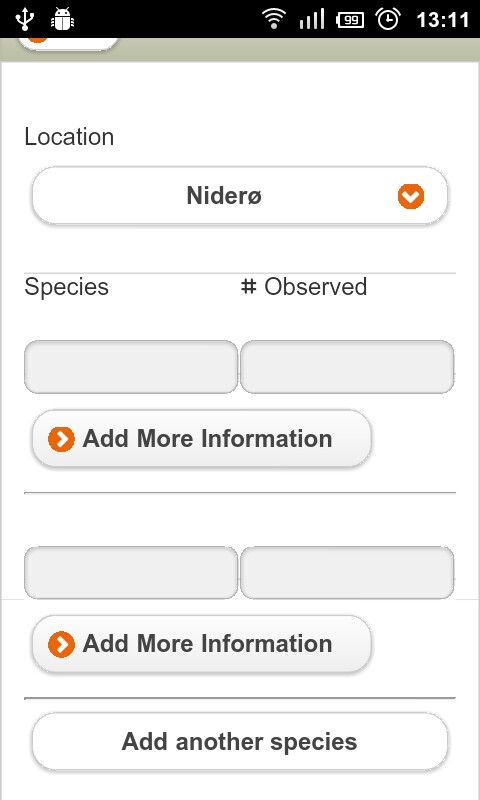
\includegraphics[width=0.5\textwidth]{sprints/ui/add_specie2.jpg}
 \end{array}$
 \end{center}
 \caption{Add Another Species, Right:Window with the new species line }
 \end{figure}
\subparagraph{Add New Species}
If the user wants to add new species he selects the “Add another species” button. This gives a new line in the same window, by adding new species the window increases its height. The user needs to slide vertically if many more species are added.  


